\documentclass[11pt,oneside,a4paper]{report}

\begin{document}
\section{Types and validation}
\label{sec:types}
The spell checking equivalent for computer programs could be type checking; a subproblem of validating a programmer's intuition of a program's intent.
Types can take properties that make them very powerful since types are, in their essence, a set of logical formulas in which we can use natural deduction to prove their validity~\cite{howard1980formulae}.
\subsection{Notation}
In the world of type theory we use natural deduction to prove type validity.
Natural deduction is expressed by \textit{inference rules}, which consist of one or more premises and a conclusion.
For instance the modus ponens rule which states that if ``if \texttt{a} implies \texttt{b} and \texttt{a}, then \texttt{b}'', can easily be written in inference rules, where \texttt{a $\rightarrow$ b} and \texttt{a} are the permises and \texttt{b} is the conclusion (\autoref{fig:not:inf}).
\begin{figure}
  \begin{mdframed}
  \begin{prooftree}
    \AxiomC{\texttt{a $\rightarrow$ b}}
    \AxiomC{\texttt{a}}
    \BinaryInfC{\texttt{b}}
  \end{prooftree}
  \end{mdframed}
  \caption{}
  \label{fig:not:inf}
\end{figure}
Conditions can also occur rules which state what conditions must be met for the rule to apply (\autoref{fig:not:notdead}).
\begin{figure}
  \begin{mdframed}
  \begin{prooftree}
    \AxiomC{\texttt{P}}
    \AxiomC{\texttt{P} is not dead}
    \BinaryInfC{\texttt{P} is alive}
  \end{prooftree}
  \end{mdframed}
  \caption{}
  \label{fig:not:notdead}
\end{figure}
Furthermore, hypotheses are written $\Gamma \vdash p$ which states that under the assumption of $\Gamma$ then $p$.

%\begin{lstlisting}[language=ML,caption={Head implementation},label={lst:headimpl},mathescape=true]
%$\texttt{fun head l: List a} \rightarrow \texttt{a =}$
    %$\texttt{match l}$
        %$\texttt{| Cons x \_ } \rightarrow \texttt{x;}$
        %$\texttt{| Nil} \rightarrow \texttt{?;}$
    %;
%\end{lstlisting}
%For instance, consider the implementation of the fuction with type $\texttt{List a} \rightarrow \texttt{a}$ in \autoref{lst:headimpl}.
%A total implementation of the function cannot exist.

%The type system for the $L$ language will be the Hindley-Milner type system~\cite{hindley1969principal,milner1978theory}.

\subsection{The language of types}
The untyped lambda calculus is exactly that, untyped.
For it to become typed, we must introduce how types occur.
A very simple type system for the how typed lambda calculus can be proved must introduce a rule for each of the lambda calculus term types Var, Let, App and Abs.
Types occur in programs, as such, programs are the assumption for a proof of such a program's types such that the assumption for types will become a set of program variables $\{x_1 \dots x_n\}$ paired with their respective type $\Gamma = \{(x_1 : \tau_1)\}, \dots (x_n : \tau_n)\}$.
Stating that it is assumed that a variable $x$ of type $\tau$ occurs in $\Gamma$ is written $\Gamma, x: \tau$

With the aforementioned knowledge, we can develop a simple set of inference rules which can be used to prove programs with types (\autoref{fig:simpletyped}).
\begin{figure}
  \begin{mdframed}
    \begin{subfigure}[b]{0.33\textwidth}
		\begin{prooftree}
			\AxiomC{$x: \tau \in \Gamma$}
			\LeftLabel{Var}
			\UnaryInfC{$\Gamma\vdash x:\tau$}
		\end{prooftree}
    \end{subfigure}
    \begin{subfigure}[b]{0.65\textwidth}
		\begin{prooftree}
			\AxiomC{$\Gamma \vdash e_1 : \tau_1 \rightarrow \tau_2$}
			\LeftLabel{App}
			\AxiomC{$\Gamma \vdash e_2 : \tau_1$}
			\BinaryInfC{$\Gamma \vdash e_1 e_2 : \tau_2$}
		\end{prooftree}
    \end{subfigure}
		\begin{prooftree}
			\AxiomC{$\Gamma, x: \tau_1 \vdash e : \tau_2$}
			\LeftLabel{Abs}
			\UnaryInfC{$\Gamma \vdash \lambda x . e : \tau_1 \rightarrow \tau_2$}
		\end{prooftree}
		\begin{prooftree}
			\AxiomC{$\Gamma \vdash e_1 : \tau_1$}
			\LeftLabel{Let}
			\AxiomC{$\Gamma ,x : \tau_1 \vdash e_2 : \tau_2$}
			\BinaryInfC{$\Gamma \vdash \texttt{let } x = e_1 \texttt{ in } e_2 : \tau_2$}
		\end{prooftree}
  \end{mdframed}
  \caption{A simple set of rules for the simply typed lambda calculus}
  \label{fig:simpletyped}
\end{figure}
\begin{itemize}
  \item Var states that if $x$ has type $\tau$ in $\Gamma$ then it is assumed that $x$ has type $\tau$.
  \item App states that if $e_1$ can be proved to have type $\tau_1 \rightarrow \tau_2$ and $e_2$ can be proved to have type $\tau_1$, then $e_1 e_2$ must be of type $\tau_2$.
  \item Abs states that if $e$ has type $\tau_2$ under the assumption that $x$ has some type $\tau_1$, then $\lambda x.e$ must be of type $\tau_1 \rightarrow \tau_2$.
  \item Let does not yet have an important role, since let does the exact same as a combination of App and Abs.
    Once polymorphism is introduced, Let will play an important role.
    Currently Let states that if $e_1$ has type $\tau_1$, and $e_2$ has type $\tau_2$ under the assumption that $x$ has type $\tau_1$ (from the proof that $e_1: \tau_1$ since $x = e_1$) then \texttt{let $x = e_1$ in $e_2$} must have inhabit the type $\tau_2$.
\end{itemize}

Before delving into types, the lambda calculus defined in \autoref{sec:lc} must be augmented with the \textit{let expression} (\autoref{eq:letb}).
\begin{align}
	\texttt{let } x = Y \texttt{ in } E
	\label{eq:letb}
\end{align}
It should be noted that the let binding can be expressed by abstraction and application (\autoref{eq:letaa}).
\begin{align}
	(\lambda x . E) (Y)
	\label{eq:letaa}
\end{align}
The let expression has a nice property that will become apparent later when typing rules are introduced.

Types are an artificial layer atop of a program just as spell checking is an artificial layer atop text.
There are two variants of types in the Hindley-Milner type system, the \textit{monotype} and the \textit{polytype}.
A monotype is either a type variable, an abstraction of two monotypes or an application of a type constructor (\autoref{eq:mono}).
\begin{align}
	mono \,\,\tau = a \,|\, \tau \rightarrow \tau \,|\, C \tau_1 \dots \tau_n
	\label{eq:mono}
\end{align}
\textit{Atoms} are terminal terms in a formula and are expressed either by type variable $a$ or $C$ with no type parameters.
The application term of the monotype is dependent on the primitive types of the programming language.
The types $\tau_1 \dots \tau_n$ are monotype parameters required to construct some type $C$.
In $L$ the set of type constructors are $\{ \texttt{Int}, \texttt{Bool} \} \cup \texttt{ADT}$.
\texttt{Int} and \texttt{Bool} are type constructors of arity 0 thus only have one instantiation and are atomic.
The set of constructors \texttt{ADT} encapsulates the set of program defined algebraic data structures (\autoref{adts}).
\begin{exmp}
    Let $\texttt{ADT} = \{ \texttt{List} \}$ where \texttt{List} is defined as in \autoref{lst:listadt}.
    The \textit{type constructor} (not to be confused for constructors like \texttt{Cons} or \texttt{Nil}) for \texttt{List} has the signature $\texttt{a} \rightarrow \texttt{List a}$ stating that if supplied with some type \texttt{a} it constructs a type of \texttt{List a} (effectively containing the provided type).
    The type \texttt{List} is a type constructor with one type parameter \texttt{a}.
\end{exmp}

$\bot$ denotes falsity, in type systems a value of this type can never exist since that in itself would disprove the program.
It is common in programming languages with strong type systems to let thrown exceptions be of type $\bot$ since it adheres to every type and indicates that the program is no longer running, since no instance of $\bot$ can exist.
$\top$ denotes truth, in type systems every type is a supertype of $\top$.
$\top$ is in practice only used to model side effects, since not all side effects return useful values.
In programming languages with side effects $\bot$ and $\top$ are considerably more useful than in pure programming languages.

A polytype is a polymorphic type (\autoref{eq:poly}).
\begin{align}
	poly \,\, \sigma = \tau \,|\, \forall a . \sigma
	\label{eq:poly}
\end{align}
Polymorphic types either take the shape of a type variable or introduce a type which all types $a$ adhere to. 
This does not necessarily include \textit{all} types since the \textbf{Gen} rule of \autoref{fig:hmrules} constrains the domain that $a$ ranges over to contain only type variables that are not free.
Many types may adhere to a polymorphic type but polymorphic types do not adhere to any type other than polymorphic types.
The concept of adherence in types is commonly called \textit{subtyping}.
Every subtype is a \textit{at least} an implementation of it's supertype.
Since this concept can be difficult to grasp from just text, observe \autoref{fig:polytree}.
\begin{figure}[ht]
    \centering
        \begin{tikzpicture}
            \node[draw=none] (sigma) {$\sigma$};

            \node[draw=none, below = of sigma] (top) {$\top$};

            \node[draw=none, below = of top] (tv) {$\tau$};
            \node[draw=none, left = of tv] (arr) {$\tau_1 \rightarrow \tau_2$};
            \node[draw=none, right = of tv] (tc) {$C \tau_1 \dots \tau_n$};

            \node[draw=none, below = of tv] (bot) {$\bot$};

            \path [->] (sigma) edge node[left] {} (top);

            \path [->] (top) edge node[left] {} (arr);
            \path [->] (top) edge node[left] {} (tv);
            \path [->] (top) edge node[left] {} (tc);

            \path [->] (tv) edge node[left] {} (bot);
            \path [->] (arr) edge node[left] {} (bot);
            \path [->] (tc) edge node[left] {} (bot);
        \end{tikzpicture}
    \caption{The type hierarchy of Hindley-Milner.}
    \label{fig:polytree}
\end{figure}
Note that $\sigma$ is controversial to introduce to the type hierarchy and has only been so to illustrate the point of subtyping.
$\sigma$ is but a mechanism to prove type systems, $\sigma$ is never a specific type.
\begin{remark}
    \label{remark:polyimpl}
An important implementation detail which should be noted is that of the polymorphic type.
Polymorphic types can be regarded as being a pair of bound types and monotype.
Instead of keeping track of what types cannot occur, keeping track of the ones than can occur simplifies the implementation.
This representation is convenient for the \textbf{Gen} rule.
\end{remark}

A principal component of typing in Hindley-Milner is the \textit{environment}.
The environment $\Gamma$ is a set of pairs of variable names and polytype (\autoref{eq:env}).
$\Gamma \vdash x: \sigma$ implies a \textit{typing judgment}, meaning that given $\Gamma$, the variable $x$ can take the type $\sigma$.
\begin{remark}
    \label{remark:judgpoly}
    Judging a type does not necessarily mean that the judged type is the only type that $x$ may take, it states that it is one \textit{possible} type that $x$ may take.
    The property of taking multiple possible types is what allows polymorphism.
    This is made more apparent in \autoref{exmp:letpoly} where \texttt{id} may take the type of either $\forall a . a \rightarrow a$, $\texttt{Int} \rightarrow \texttt{Int}$ or $\forall a . (a \rightarrow a) \rightarrow (a \rightarrow a)$.
\end{remark}
\begin{align}
	\Gamma \,\, = \epsilon \,|\, \Gamma, x : \sigma
	\label{eq:env}
\end{align}

Like in the untyped lambda calculus, types also have notions of free and bound type variables.
Bound type variables are ones that explicitly have been introduced to the type system by either let or abstraction in the context of some expression.
Type variables are bound when they have been introduced by a quantification or exist in the environment.
\begin{align}
	 & \textit{free}(a) = \{ a \}                                                              \\
	 & \textit{free}(C \tau_1 \dots \tau_n ) = \bigcup_{i = 1}^n \textit{free}(\tau_i)           \\
     & \textit{free}(\tau_1 \rightarrow \tau_2) = \textit{free}(\tau_1) \cup \textit{free}(\tau_2)          \\
	 & \textit{free}(\Gamma) = \bigcup_{x:\sigma \in \Gamma} \textit{free}(\sigma)             \\
	 & \textit{free}(\forall a . \sigma) = \textit{free}(\sigma) - \{ a \}                     
	 %& \textit{free}(\Gamma \vdash x : \sigma) = \textit{free}(\sigma) - \textit{free}(\Gamma)
\end{align}
\begin{exmp}
Consider the type for the function \texttt{fst} in \autoref{lst:fstimpl}.
\begin{lstlisting}[language=ML,caption={First function},label={lst:fstimplbad},mathescape=true]
fun fst a b: $\forall$A.$\forall$B.A $\rightarrow$ B $\rightarrow$ A = a;
\end{lstlisting}
\begin{lstlisting}[language=ML,caption={First function in lambda calculus},label={lst:fstimpl},mathescape=true]
let fst = $\lambda$a.(let f = $\lambda$b.a in f) in fst
\end{lstlisting}
    The type for \texttt{fst} is $\forall A \forall B . A \rightarrow B \rightarrow A$.

    Note that a naive typing could look like $\forall A  . A \rightarrow (\forall B . B \rightarrow A)$ but rank-2 polymorphism is not typable in Hindley-Milner.
    An important realization is the context from where the type analysis is made.
    If type analysis is made from within the bounded context of \texttt{f} the type of \texttt{f} becomes $\forall B . B \rightarrow A$ and the type variable $A$ is free.
\end{exmp}
The variables which may appear in a quantification have an important role in \autoref{eq:substitution}, since only free variables may be substituted.
Free variables are also a core part of generalizing a type for inference algorithms (\autoref{subsec:algw}).
When modelling polymorphic types with a technique such as \autoref{remark:polyimpl} finding the set of bound variables is trivial.
\begin{align}
    & \textit{bound}(\tau) = \textit{free}(\tau) - \textit{free}(\Gamma)
\end{align}
When generalizing a type $\tau$ all types which do not occur in $\Gamma$ must be quantified.
\begin{exmp}
\begin{gather}
    \Gamma = \{ (\textit{x}, \gamma) \} \label{eq:monoeq}\\
\begin{align}
    \textit{bound}(\tau \rightarrow \gamma) &= \{\tau , \gamma\} - \textit{free}(\Gamma)\\
    &= \{\tau , \gamma\} - \{ \gamma \} = \{ \tau \}\tag*{}
\end{align}
\end{gather}
Clearly the only bound type variable in the context of $\tau \rightarrow \gamma$ is $\tau$ such that it may become $\forall \tau. \tau \rightarrow \gamma$ in the instance that the type represents a polymorphic let expression.
    Note that $\texttt{x:}\gamma$ in \autoref{eq:monoeq} does not contain $\gamma$ as a quantified type since it has been introduced by an abstraction and \textbf{Abs} only introduces monomorphic types (\autoref{fig:hmrules}).
    An interesting observation is that there can only exist one implementation of the above type system if $\tau \rightarrow \gamma$ is to be introduced by a polymorphic let expression which is displayed in \autoref{lst:theoremsforfree}~\cite{wadler1989theorems}.
\begin{lstlisting}[language=ML,caption={Implementation of type state},label={lst:theoremsforfree},mathescape=true]
$\lambda$x.
    let z = ($\lambda$y.x) in
    $\dots$
\end{lstlisting}
\end{exmp}

\section{Hindley-Milner}
With the now introduced primitives, the Hindley-Milner type system is but a set of rules composed by said primitives.
\begin{figure}[ht]
	\begin{mdframed}
		\begin{prooftree}
			\AxiomC{$x: \sigma \in \Gamma$}
			\LeftLabel{Var}
			\UnaryInfC{$\Gamma\vdash x:\sigma$}
		\end{prooftree}
		\begin{prooftree}
			\AxiomC{$\Gamma \vdash e_1 : \tau_1 \rightarrow \tau_2$}
			\LeftLabel{App}
			\AxiomC{$\Gamma \vdash e_2 : \tau_1$}
			\BinaryInfC{$\Gamma \vdash e_1 e_2 : \tau_2$}
		\end{prooftree}

		\begin{prooftree}
			\AxiomC{$\Gamma, x: \tau_1 \vdash e : \tau_2$}
			\LeftLabel{Abs}
			\UnaryInfC{$\Gamma \vdash \lambda x . e : \tau_1 \rightarrow \tau_2$}
		\end{prooftree}
		\begin{prooftree}
			\AxiomC{$\Gamma \vdash e_1 : \sigma$}
			\LeftLabel{Let}
			\AxiomC{$\Gamma ,x : \sigma \vdash e_2 : \tau$}
			\BinaryInfC{$\Gamma \vdash \texttt{let } x = e_1 \texttt{ in } e_2 : \tau$}
		\end{prooftree}

		\begin{prooftree}
			\AxiomC{$\Gamma \vdash e : \sigma_1$}
			\AxiomC{$\sigma_1 \sqsubseteq \sigma_2$}
			\LeftLabel{Inst}
			\BinaryInfC{$\Gamma \vdash e : \sigma_2$}
		\end{prooftree}
		\begin{prooftree}
			\AxiomC{$\Gamma \vdash e : \sigma$}
            \AxiomC{$a \notin \textit{free}(\Gamma)$}
			\LeftLabel{Gen}
			\BinaryInfC{$\Gamma \vdash e : \forall a . \sigma$}
		\end{prooftree}
	\end{mdframed}
	\caption{Hindley-Milner type rules}
	\label{fig:hmrules}
\end{figure}
There are six rules in the Hindley-Milner rules outlined in \autoref{fig:hmrules}.
\begin{itemize}
    \item \textbf{Var} states that if some variable $x$ with type $\sigma$ exists in the environment, the type can be judged.
        In practice, when $x: \sigma$ is encountered in the expression tree it is added to the environment.
    \item \textbf{App} decides that if $e_1 : \tau_1 \rightarrow \tau_2$ and $e_2 : \tau_1$ has been judged to exist then $e_1 e_2$ implies the removal of $\tau_1$ from $\tau_1 \rightarrow \tau_2$ such that $e_1 e_2: \tau_2$.
    \item \textbf{Abs} is the typing rule of lambda abstractions.
        If $x : \tau_1$ exists in the environment from some type analysis of $e$ and the abstraction's body $e$ has been judged to be of type $\tau_2$ then the abstraction of $x$ must take the type of $x$ to create the type of the body $e$.
    \item \textbf{Let} states that if $e_1$ has been judged to have type $\sigma$ then the let expression's identifier $x: \sigma$ must exist in the environment when deriving the type of $e_2$.
        Observe that \textbf{Let} introduces a polymorphic type to the environment while \textbf{Abs} introduces a monomorphic one.
        Note that by \autoref{remark:judgpoly} $x$ may be polymorphic in $e_2$.
    \item \textbf{Inst} specializes some polymorphic type (in regard to the type system implementation) to a more specific polymorphic type.
        $\sqsubseteq$ is the partial order of types where the binary relation between two types compares the descriptiveness of types.
        \begin{exmp}
            In $L$ the smallest element is the top of the type hierarchy (\autoref{fig:polytree}), the polymorphic type.
        \end{exmp}
    \item \textbf{Gen} generalizes over all bound variables $a$.
\end{itemize}
Let polymorphism is exemplified in \autoref{exmp:letpoly}.

\begin{exmp}
\label{exmp:letpoly}
Throughout this example the convenient syntax $(x, z)$ is the pair of the variables $x$ and $z$ which can be implemented by algebraic data structures or a combinator.

The identity function is a common example to illustrate type systems (\autoref{lst:idfun}).
\begin{lstlisting}[language=ML,caption={Identity function in $L$},label={lst:idfun}]
fun id x = x;
id 4;
\end{lstlisting}
\begin{lstlisting}[language=ML,caption={Identity function in lambda calculus with let},label={lst:idfunlam},mathescape=true]
let id = ($\lambda x . x$) in
id 4
\end{lstlisting}
Stating that id has the type $\forall a.a \rightarrow a$ and $4$ has the type \texttt{Int} is \autoref{lst:idfunlam} program correct?
By applying the Hindley-Milner rules one can prove or disprove this statement.
A correct proof of \autoref{lst:idfun} must be \autoref{fig:typeexampleid}.

\begin{lstlisting}[language=ML,caption={Identity function in lambda calculus by abstraction},label={lst:idfunlamabs},mathescape=true]
($\lambda$id.id 4)($\lambda$x.x)
\end{lstlisting}
\autoref{lst:idfunlam} and \autoref{lst:idfunlamabs} are two equivalent programs with slightly different proofs which raises the question of why the let expression is even needed.
If \autoref{lst:idfunlam} and \autoref{lst:idfunlamabs} were to be slightly changed such that two new programs \autoref{lst:idfunlam2} and \autoref{lst:idfunlamabs2} were to be proved, \autoref{lst:idfunlamabs2} would not be provable while \autoref{lst:idfunlam2} would.
\begin{lstlisting}[language=ML,caption={Identity function with two applications},label={lst:idfunlam2},mathescape=true]
let id = ($\lambda$x.x) in
(id 4, id id)
\end{lstlisting}
\begin{lstlisting}[language=ML,caption={Identity function with two applications as abstraction},label={lst:idfunlamabs2},mathescape=true]
($\lambda$id.(id 4, id id)($\lambda$x.x)
\end{lstlisting}
In \autoref{lst:idfunlamabs2} \texttt{id} cannot adhere to polymorphism by \textbf{Abs} in \autoref{fig:hmrules} whilst \textbf{Let} can.
%\begin{figure}[ht]
    %\begin{mdframed}[style=bigbox]
        %\begin{subfigure}[b]{1\textwidth}
        %\begin{prooftree}
                            %\AxiomC{$x : a \in \Gamma$}
                            %\LeftLabel{Var}
                        %\UnaryInfC{$\Gamma \vdash x : a$}
                    %\LeftLabel{Abs}
                %\UnaryInfC{$\Gamma \vdash (\lambda x . x) : a \rightarrow a$}
                    %\LeftLabel{Gen}
                    %\AxiomC{$a \notin \textit{free}(\Gamma)$}
                %\BinaryInfC{$\Gamma \vdash (\lambda x . x) : \forall a . a \rightarrow a$}
                %\AxiomC{$\forall a . a \rightarrow a \sqsubseteq \texttt{Int} \rightarrow \texttt{Int}$}
            %\LeftLabel{Inst}
            %\BinaryInfC{$\Gamma \vdash (\lambda x . x) : \texttt{Int} \rightarrow \texttt{Int}$}
        %\end{prooftree}
        %\caption{}
        %\label{fig:typewrongexampleid:1}
        %\end{subfigure}
        %\begin{subfigure}[b]{0.49\textwidth}
        %\begin{prooftree}
                    %\AxiomC{$\text{id} : \texttt{Int} \rightarrow \texttt{Int} \in \Gamma$}
                    %\LeftLabel{Var}
                %\UnaryInfC{$\Gamma \vdash \text{id} : \texttt{Int} \rightarrow \texttt{Int}$}
                    %\AxiomC{$4 : \texttt{Int} \in \Gamma$}
                    %\RightLabel{Var}
                %\UnaryInfC{$\Gamma \vdash 4 : \texttt{Int}$}
            %\RightLabel{App}
            %\BinaryInfC{$\Gamma, \text{ id} : \texttt{Int} \rightarrow \texttt{Int} \vdash $ id 4 : \texttt{Int}}
        %\end{prooftree}
        %\caption{}
        %\label{fig:typewrongexampleid:2}
        %\end{subfigure}
        %\begin{subfigure}[b]{0.49\textwidth}
        %\begin{prooftree}
                %\AxiomC{\ref{fig:typewrongexampleid:1}}
                %\AxiomC{\ref{fig:typewrongexampleid:2}}
            %\LeftLabel{Let}
            %\BinaryInfC{$\Gamma \vdash $ \texttt{let} id = $(\lambda x . x)$ \texttt{in} id 4: \texttt{Int}}
        %\end{prooftree}
        %\caption{}
        %\label{fig:typewrongexampleid:3}
        %\end{subfigure}
    %\end{mdframed}
    %\caption{Incorrect identity function instantiation proof}
    %\label{fig:typewrongexampleid}
%\end{figure}
\begin{figure}[ht]
    \begin{mdframed}[style=bigbox]
        \begin{subfigure}[b]{1\textwidth}
        \begin{prooftree}
                            \AxiomC{$\text{id} : \forall a . a \rightarrow a \in \Gamma$}
                            \LeftLabel{Var}
                        \UnaryInfC{$\Gamma \vdash \text{id} : \forall a . a \rightarrow a$}
                        \AxiomC{$\forall a . a \rightarrow a \sqsubseteq \texttt{Int} \rightarrow \texttt{Int}$}
                    \LeftLabel{Inst}
                    \BinaryInfC{$\Gamma \vdash \text{id} : \texttt{Int} \rightarrow \texttt{Int}$}
                        \AxiomC{$4 : \texttt{Int} \in \Gamma$}
                        \RightLabel{Var}
                    \UnaryInfC{$\Gamma \vdash 4 : \texttt{Int}$}
                \RightLabel{App}
                \BinaryInfC{$\Gamma, \text{ id} : \forall a . a \rightarrow a \vdash $ id 4 : \texttt{Int}}
        \end{prooftree}
        \caption{}
        \label{fig:typeexampleid:2}
        \end{subfigure}
        \begin{subfigure}[b]{0.49\textwidth}
        \begin{prooftree}
                                \AxiomC{$x : a \in \Gamma$}
                                \LeftLabel{Var}
                            \UnaryInfC{$\Gamma \vdash x : a$}
                        \LeftLabel{Abs}
                    \UnaryInfC{$\Gamma \vdash (\lambda x . x) : a \rightarrow a$}
                        \LeftLabel{Gen}
                        \AxiomC{$a \notin \textit{free}(\Gamma)$}
                    \BinaryInfC{$\Gamma \vdash (\lambda x . x) : \forall a . a \rightarrow a$}
        \end{prooftree}
        \caption{}
        \label{fig:typeexampleid:1}
        \end{subfigure}
        \begin{subfigure}[b]{0.49\textwidth}
        \begin{prooftree}
                \AxiomC{\ref{fig:typeexampleid:1}}
                \AxiomC{\ref{fig:typeexampleid:2}}
            \LeftLabel{Let}
            \BinaryInfC{$\Gamma \vdash $ \texttt{let} id = $(\lambda x . x)$ \texttt{in} id 4: \texttt{Int}}
        \end{prooftree}
        \caption{}
        \label{fig:typeexampleid:3}
        \end{subfigure}
    \end{mdframed}
    \caption{Identity function instantiation proof}
    \label{fig:typeexampleid}
\end{figure}
\end{exmp}



\subsection{Damas-Milner Algorithm W}
\label{subsec:algw}
Typing rules are by themselves not that useful since they need all type information declared ahead of checking, inference attempts to guess types such that the rules are satisfied.
Type inference is the technique of automatically deriving types, of which there exist many algorithms.
One of the most common inference algorithms that produce typings which the Hindley-Milner rules accept is the Damas-Milner Algorithm W inference algorithm~\cite{damas1984type,damas1982principal}.

The Damas-Milner Algorithm W rules (\autoref{fig:dmrules}) introduce some new concepts such as \textit{fresh variables}, \textit{most general unifier}, and the \textit{substitution set}.
Fresh variables are introduced by picking a variable that has not been picked before from the infinite set $\tau_1, \tau_2 \dots $.
Fresh variables are introduced when unknown types are discovered and later unified.
The substitution set is a mapping from type variables to types (\autoref{eq:substitution}).
\begin{align}
    S = \{ a_1 \mapsto \tau_1, a_2 \mapsto \tau_2 \dots , a_n \mapsto \tau_n \} 
    \label{eq:substitution}
\end{align}
A substitution written $S T$ where $T$ is an arbitrary component of Hindley-Milner like an environment in which all type variables are substituted (\autoref{fig:subsem}).
\begin{figure}
\begin{mdframed}
\begin{align}
    &S \Gamma = \{ (x, S \sigma) \,\,|\,\, \forall (x, \sigma) \in \Gamma \} \tag{Environment}\\
    &S \sigma  = 
        \begin{cases}
            S \tau & \text{if } \sigma \equiv \tau\\
            \{ a' \mapsto \tau_1 \,\,|\,\, (a', \tau_1) \in S \,\,|\,\, (a, *) \notin S \} \sigma' & \text{if } \sigma \equiv \forall a . \sigma'
        \end{cases}
    \tag{Poly}\\
    &S (\tau_1 \rightarrow \tau_2) = S\tau_1 \rightarrow S\tau_2 \tag{Arrow}\\
    &S a = 
        \begin{cases}
            \tau & \text{if } (a, \tau) \in S\\
            a & 
        \end{cases}
    \tag{Typevariable}\\
    &S C \tau_1 \dots \tau_n = C S\tau_1 \dots S\tau_n \tag{Constructor}
\end{align}
\end{mdframed}
    \caption{Substitution semantics}
    \label{fig:subsem}
\end{figure}
Substitution sets can also be combined $S_1 \cdot S_2$ with well defined-semantics.
The combination of substitution sets is a key component for the correctness of the Damas-Milner inference algorithm.
\begin{align}
    S_1 \cdot S_2 = \{ (a \mapsto S_1\tau) \,\,|\,\, (a \mapsto \tau) \in S_2) \} \cup S_1
    \label{eq:combination}
\end{align}
\begin{remark}
By the substitution set combination operator transitive and circular substitutions cannot occur since type variables in $S_1$ will inherit all the mappings from $S_2$ by union.
Trasitivity is avoided by substituting all instances of type variables values (the mapped to type variables) in $S_2$ with ones that occur in $S_1$.
The properties ensured by the combination semantics also induce the property of idempotence.
This property is enforced by the Damas-Milner Algorithm W inference rules.
\end{remark}
Unification is performed differently based on the context.
Unification is performed on monotypes, each of which can take one of three forms (\autoref{eq:mono}).
Note that the Var rules for most general unifier outlined in \autoref{fig:mgu} are commutative.
\begin{figure}
	\begin{mdframed}
		\begin{prooftree}
			\AxiomC{$S, \{ (\tau_1 \rightarrow \tau_2, \gamma_1 \rightarrow \gamma_2) \} \cup T $}
			\LeftLabel{Arrow}
			\UnaryInfC{$S,T \cup \{ (\tau_1, \gamma_1), (\tau_2, \gamma_2) \}$}
		\end{prooftree}

		\begin{prooftree}
            \AxiomC{$\tau_1, \tau_2$}
            \LeftLabel{Intro}
			\UnaryInfC{$\emptyset, \{ (\tau_1, \tau_2) \}$}
		\end{prooftree}
		\begin{prooftree}
			\AxiomC{$S, \{ (a, \tau_1) \} \cup T$}
			\AxiomC{$a \equiv \tau_1$}
			\LeftLabel{
				Var empty
			}
			\BinaryInfC{$S, T $}
		\end{prooftree}

		\begin{prooftree}
			\AxiomC{$S, \{ (a, \tau_1) \} \cup T $}
			\AxiomC{$a \notin \textit{free}(\tau_1)$}
			\LeftLabel{Var sub}
			\BinaryInfC{$S \cup \{ a \mapsto S\tau_1 \}, \{ a \mapsto S\tau_1 \} \cup T$}
		\end{prooftree}

		\begin{prooftree}
			\AxiomC{$S,C_1 \tau_1 \dots \tau_n,C_2 \gamma_1 \dots \gamma_n \cup T$}
			\AxiomC{$C_1 \equiv C_2$}
			\LeftLabel{Atom}
			\BinaryInfC{$S , \{ (\tau_1, \gamma_1) \dots , (\tau_n, \gamma_n)\} \cup T$}
		\end{prooftree}
	\end{mdframed}
	\caption{Rules for most general unification}
	\label{fig:mgu}
\end{figure}

%\begin{lemma}
	%Var sub and Var empty are commutative.
%\end{lemma}
%\begin{proof}
	%Var empty is trivially true since $\equiv$ is commutative and for any $a$ and $\tau_1$ the rule produces $\emptyset \cup T = T$.\\\\
    %The commutative property of Var sub comes from the realization that $S \cup \{ \tau_1 \mapsto S\tau_2 \}$ and $S \cup \{ \tau_2 \mapsto S\tau_1 \}$ lets Algorithm W accept on the same inputs.
    %Furthermor note that Algorithm W substitutes and combines substitution sets at every step of the expression tree such that transitive types never occur because of the combination semantics.
    %\begin{case}
        %The types $\tau_1$ and $\tau_2$ are first introduced and used in unification.
        %Either all future uses of $\tau_1$ will be mapped to $\tau_2$ by the substitution set or all future uses of $\tau_2$ will be mapped to $\tau_1$.
    %\end{case}
    %\begin{case}
        %$\tau_1$ has been assigned in an earlier unification.
        %If $\tau_2 \mapsto \tau_1$ any existing references to $\tau_1$ need not change since all expressions of type variable $\tau_2$ will be mapped by the rules defined in \autoref{fig:hmrules}.
        %If any future rules need the type variable $\tau_1$ and $\tau_1 \mapsto \tau_2$ is introduced to the substitution set, the substitution rules in \autoref{fig:hmrules} will substitute the type.
    %\end{case}
%\end{proof}
\begin{remark}
    The Damas-Milner algorithm W is the most popular inference algorithm for Hindley-Milner.
    Though it remains the most popular, it has some interesting competitors.
    One of which is that of the constraint solver approach which is also used in OCaml~\cite{heeren2002generalizing}.
    The constraint solver approach is a two phase type inference algorithm.
    In the first phase the algorithm inspects the expression tree and generates a set of constraints as it goes.
    After the set of constraints $C$ has been generated it then traverses the constraints and generates type variable substitutions.
    It is argued that error reporting is significantly easier in such an approach.
\end{remark}
\begin{figure}[ht]
	\begin{mdframed}[style=style1]
		\begin{prooftree}
			\AxiomC{$x: \sigma \in \Gamma$}
			\AxiomC{$\tau = \textit{inst}(\sigma)$}
			\LeftLabel{Var}
			\BinaryInfC{$\Gamma \vdash x:\tau , \emptyset$}
		\end{prooftree}
		\begin{prooftree}
			\AxiomC{$\tau_1 = \textit{fresh}$}
			\AxiomC{$\Gamma, x: \tau_1 \vdash e: \tau_2, S$}
			\LeftLabel{Abs}
			\BinaryInfC{$\Gamma \vdash \lambda x . e : S\tau_1 \rightarrow \tau_2, S$}
		\end{prooftree}

		\begin{center}
			App
		\end{center}
		\vspace{-0.7cm}
		\begin{prooftree}
			\AxiomC{$\Gamma \vdash e_1 : \tau_1, S_1 \,\,\,\, \tau_3 = \textit{fresh}$}
			\AxiomC{$S_1 \Gamma \vdash e_2 : \tau_2, S_2 \,\,\,\, S_3 = \textit{mgu}(S_2 \tau_1, \tau_2 \rightarrow \tau_3)$}
			\BinaryInfC{$\Gamma \vdash e_1 e_2 : S_3 \tau_3, S_3 \cdot S_2 \cdot S_1$}
		\end{prooftree}

		\begin{prooftree}
			\AxiomC{$\Gamma \vdash e_1 : \tau_1, S_1$}
			\AxiomC{$S_1 \Gamma , x : S_1 \Gamma(\tau_1) \vdash e_2 : \tau_2, S_2$}
			\LeftLabel{Let}
			\BinaryInfC{$\Gamma \vdash \texttt{let } x = e_1 \texttt{ in } e_2 : \tau_2, S_1 \cdot S_2$}
		\end{prooftree}
	\end{mdframed}
	\caption{Algorithm W}
	\label{fig:dmrules}
\end{figure}
\begin{remark}
In the language $L$ a function \texttt{fun} translates to a let expressions while \texttt{let} translates to abstraction and application.
\end{remark}
\subsection{Instantiation}
Another interesting addition introduced by algorithm W in \autoref{fig:dmrules} is \textit{inst}.
\textit{inst} naturally follows from the \textbf{Inst} rule in \autoref{fig:hmrules} but has a slightly different behaviour.
The \textit{inst} function does not specify types anymore but simply makes unification of polymorphic types possible.
\begin{align}
    &\textit{inst}(\sigma) = \{ \, a \mapsto \textit{fresh} \,\,|\,\, a \notin \textit{free}(\sigma) \, \}\sigma
    \label{eq:inst}
\end{align}
\textit{inst} (\autoref{eq:inst}) maps all bound type variables to fresh type variables in the polytype $\sigma$.
\textit{inst} is an important component to allow polymorphic types to remain polymorphic since no bound type variables may be substituted.
\begin{exmp}
    Performing some type analysis on \autoref{lst:polyid} yields a very rich example of why \textit{inst} is necessary.
    \newline
    \begin{minipage}{\textwidth}
\begin{lstlisting}[language=ML,caption={Polymorphic id},label={lst:polyid},mathescape=true]
fun id x = x;
fun ap x f = f x;
fun doubleid x = id (id (x + 1));
\end{lstlisting}
    \end{minipage}
    After inferring \texttt{id} and \texttt{ap} the environment will contain id $\Gamma = \{ (\texttt{id}, \forall a . a \rightarrow a), (\texttt{ap}, \forall \gamma,\beta . \gamma \rightarrow (\gamma \rightarrow \beta) \rightarrow \beta)\}$.
    Typing the function \texttt{doubleid} without the use of \textit{inst}; begin by looking at the introduced parameter \texttt{x} and then the innermost expression \texttt{id (x + 1)}. 
\begin{align}
    &\textit{bound}(\tau) = \textit{free}(\tau) - \textit{free}(\Gamma) = \{ \tau \} \tag{\textbf{Abs} intro \texttt{x} : $\tau$ }\\
    &\Gamma = \{ (\texttt{id}, \forall a . a \rightarrow a), (\texttt{ap}, \forall \gamma,\beta . \gamma \rightarrow (\gamma \rightarrow \beta) \rightarrow \beta), (\texttt{x}, \forall \tau . \tau) \}\\
    &\textit{unify}(\tau, \texttt{Int}) = \{ \tau \mapsto \texttt{Int} \}\\
    &\textit{unify}(a \rightarrow a, \texttt{Int} \rightarrow \mu) = \textit{unify}(\{ a \mapsto \texttt{Int} \}a, \{ a \mapsto \texttt{Int} \}\mu) \cdot \{ a \mapsto \texttt{Int} \}\\
    &= \{ \mu \mapsto \texttt{Int} \} \cdot \{ a \mapsto \texttt{Int} \} \tag*{}\\
    &= \{ \mu \mapsto \texttt{Int}, a \mapsto \texttt{Int} \} \tag*{}
    \label{eq:unifyres}
\end{align}
    This example might not look compromising but a minor change such that the body of \texttt{doubleid} becomes \texttt{id (ap (id (x + 1)))} yields an interesting problem.
    In the case of introducing \texttt{ap} the two type instances for \texttt{id} must be different (\texttt{id} must be introduced with different type variables) to retain it's polymorphic properties.
    The following steps are performed when inferring this new body.
\begin{align}
    &\textit{unify}(\gamma \rightarrow (\gamma \rightarrow \beta) \rightarrow \beta, \texttt{Int} \rightarrow \delta) \tag{\texttt{ap (id (x + 1))} }\\
    & = \{ \gamma \mapsto \texttt{Int}, \delta \mapsto (\texttt{Int} \rightarrow \beta) \rightarrow \beta \} \tag*{}\\
    &\{ \gamma \mapsto \texttt{Int}, \delta \mapsto (\texttt{Int} \rightarrow \beta) \rightarrow \beta \} \cdot \{ \mu \mapsto \texttt{Int}, a \mapsto \texttt{Int} \} \tag{\textbf{App} $S_3 \cdot S_2$ }\\
    & = \{ \gamma \mapsto \texttt{Int}, \delta \mapsto (\texttt{Int} \rightarrow \beta) \rightarrow \beta, \mu \mapsto \texttt{Int}, a \mapsto \texttt{Int} \} \tag*{}\\
    &\textit{unify}(a \rightarrow a, ((\texttt{Int} \rightarrow \beta) \rightarrow \beta) \rightarrow \theta) \tag{\texttt{id (ap (id (x + 1)))} }\\
    &= \textit{unify}(
     \{ a \mapsto  (\texttt{Int} \rightarrow \beta) \rightarrow \beta \} a,
     \{ a \mapsto  (\texttt{Int} \rightarrow \beta) \rightarrow \beta\} \theta
    ) \cdot \{ a \mapsto  (\texttt{Int} \rightarrow \beta) \rightarrow \beta\} \tag*{}\\
    &= \{ a \mapsto (\texttt{Int} \rightarrow \beta) \rightarrow \beta, \theta \mapsto (\texttt{Int} \rightarrow \beta) \rightarrow \beta \} \cdot \{ a \mapsto (\texttt{Int} \rightarrow \beta) \rightarrow \beta\} \tag*{}\\
    &= \{ a \mapsto (\texttt{Int} \rightarrow \beta) \rightarrow \beta, \theta \mapsto (\texttt{Int} \rightarrow \beta) \rightarrow \beta \} \tag*{}\\
    &\{ a \mapsto (\texttt{Int} \rightarrow \beta) \rightarrow \beta, \theta \mapsto (\texttt{Int} \rightarrow \beta) \rightarrow \beta \} \cdot \tag{\textbf{App} $S_3 \cdot S_2$ }\\
    &\{ \gamma \mapsto \texttt{Int}, \delta \mapsto (\texttt{Int} \rightarrow \beta) \rightarrow \beta, \mu \mapsto \texttt{Int}, a \mapsto \texttt{Int} \} \tag*{}
\end{align}
    Clearly $a$ cannot map to two types which cannot be unified which is a violation of the type system.
    The apparent problem is that \texttt{id} is specialized within the whole of \texttt{doubleid}.
    By instantiating quantified types when they are needed cases such as this can be avoided (it also makes the algorithm correct).
    \begin{align}
        &\textit{unify}(\textit{inst}(\forall a . a \rightarrow a), \textit{inst}(\forall \tau . \tau \rightarrow \mu))\\
        & = \textit{unify}(\gamma \rightarrow \gamma, \varphi \rightarrow \mu) \tag*{}\\
        & = \{ \varphi \mapsto \mu, \gamma \mapsto \mu \} \tag*{}
    \end{align}
\end{exmp}
\subsection{Recursion}
Recursion is a trivial matter once the primitives of the Hindley-Milner type system have been introduced.
Recall that in \autoref{sec:lamrec} recursion (along with mutual recursion) was shown to be implementable by introducing functions to their own scope, the same is true for types.
Allowing recursive functions in Hindley-Milner type inference systems is a matter of letting the function be present in the environment when inferring the function's own body.
\begin{exmp}
If the function \texttt{f} defined in \autoref{lst:recplus1} were to be typed it would need to be introduced as an unknown type to the environment before typing the body of \texttt{f}.
\begin{lstlisting}[language=ML,caption={Recursive function},label={lst:recplus1},mathescape=true]
fun f x = (f x) + 1;
\end{lstlisting}
Let $\Gamma = \{ \texttt{f} : \forall \tau . \tau, \texttt{x} : \forall \mu . \mu \}$.
From the application \texttt{f x} the unification \texttt{unify}$(\tau, \gamma \rightarrow \mu) = \{ \tau \mapsto \mu \rightarrow \gamma \}$ must be performed, and the resulting type for the expression is $\gamma$.
The addition operation forces \texttt{unify}$(\texttt{Int}, \gamma) = \{ \gamma \mapsto \texttt{Int} \}$.
Finally the application of the addition function $+: \texttt{Int} \rightarrow \texttt{Int} \rightarrow \texttt{Int}$ and the two expressions \texttt{f x} and $1$ such that the resulting expression type is \texttt{Int}.

\end{exmp}

\subsection{Additional language features}
In addition to the rules in \autoref{fig:dmrules} many other ergonomic features can easily be modelled once the framework has been understood.
One of the most crucial features of languages are that of decision.
\begin{lstlisting}[language=ML,caption={ADT implementation of decision},label={lst:adtdecision},mathescape=true]
type Boolean = 
    | BFalse
    | BTrue
;
let b = BFalse;
fun double x = x + x;
b (0) (double 10);
\end{lstlisting}
Decision can be implemented in a variety of ways such as in \autoref{lst:adtdecision} by the use of algebraic data structures aligning very much with Church Booleans~\cite{church1985calculi}.
\begin{figure}[ht]
	\begin{mdframed}[style=bigbox]
        \begin{subfigure}[b]{1\textwidth}
            \begin{prooftree}
                \AxiomC{$\Gamma \vdash e_2 : \tau_2, S_2 \,\,\, \tau_4 = \textit{fresh} \,\,\, \Gamma, S_4 = \textit{mgu}(S_1'\cdot S_2 \cdot S_3 \tau_2, \tau_4)$}
            \end{prooftree}
            \caption{}
            \label{subfig:pt1}
        \end{subfigure}
        \begin{subfigure}[b]{0.33\textwidth}
            \begin{prooftree}
                \AxiomC{$\Gamma \vdash e_1 : \tau_1, S_1 \,\, S_1' = \textit{mgu}(\texttt{Bool}, \tau_1)$}
            \end{prooftree}
            \caption{}
            \label{subfig:pt0}
        \end{subfigure}
        \begin{subfigure}[b]{0.66\textwidth}
            \begin{prooftree}
                \AxiomC{$\Gamma \vdash e_3 : \tau_3, S_3 \,\,\, \Gamma, S_5 = \textit{mgu}(S_4 \cdot S_1'\cdot S_2 \cdot S_3 \tau_3, S_4 \tau_4)$}
            \end{prooftree}
            \caption{}
            \label{subfig:pt2}
        \end{subfigure}
        \begin{prooftree}
                \AxiomC{\ref{subfig:pt0}}
                    \AxiomC{\ref{subfig:pt1}}
                    \AxiomC{\ref{subfig:pt2}}
                \BinaryInfC{$\Gamma, S_6 \,\,\, S_6 = S_5 \cdot S_4 \cdot S_1'\cdot S_2 \cdot S_3$}
            \BinaryInfC{$\Gamma \vdash \texttt{if } e_1 \texttt{ then } e_2 \texttt{ else } e_3: S_6\tau_4, S_6$}
        \end{prooftree}
	\end{mdframed}
	\caption{Decision}
	\label{fig:decision}
\end{figure}
Rather decision can be implemented by more conventional methods than combinator logic by introducing more inference rules as in \autoref{fig:decision}.
Additional language syntax features can in most cases be implemented as decision can.
\subsection{Algebraic data structures}
To implement rules for algebraic data structures one must first decide on what the type of an algebraic data structure is.
If algebraic data structures were implemented as in \autoref{sec:adt} the type of an algebraic data structure like Boolean in \autoref{lst:adtdecision} would be \texttt{a -> a -> a} since \texttt{BFalse} and \texttt{BTrue} must have a handler each.
Implementing algebraic data structures by this method does not introduce anything to the inference algorithm since every algebraic data structure becomes a function.
It is more common to introduce algebraic data structures as new type constructor types since such an implementation yields descriptive errors in comparison to generated function types.
Fortunately type constructors are trivial to model in Hindley-Milner since a type constructor is a type lambda and rank-1 type lambdas are simply quantified types.
\autoref{lst:listadt} introduces the type constructor \texttt{a $\rightarrow$ List a} with value constructors \texttt{Cons: $\forall$a.a $\rightarrow$ List a $\rightarrow$ List a} and \texttt{Nil: $\forall$a.List a}.
For instance let some program be \texttt{Cons 1 (Cons 2 Nil)} such that inference becomes a matter of first unifying the type of \texttt{Cons} and \texttt{$\forall$a.Int $\rightarrow$ List a $\rightarrow \tau_1$} using the application rule and then unifying \texttt{$\forall$a.Int $\rightarrow \tau_1 \rightarrow \tau_2$} with \texttt{Cons} again by application.


\section{The cost of expressiveness}
Modern languages with strong type systems tend to be notoriously slow to type on pathological inputs.
In fact, many languages with strong type systems provide type systems expressive enough to be Turing-complete.

In the construction of the compiler for $L$, one target was the C++ language.
An instance of a pathological input for the C++ type checker is most definitely the untyped lambda calculus.
The lambda terms in C++ must adhere to polymorphism in many cases which leads to some unknown but large blowup in compilation time.
In fact type polymorphism is commonly the root of blowup in typing.

ML, which implements a Hindley-Milner inference system, was believed to have linear complexity before shown to be exponential along with other problematic complexity findings~\cite{mairson1989deciding}.
As it will turn out, Hindley-Milner also suffers an explosive worst case induced by a pathological input fueled by polymorphism.

\begin{lemma}
    There exists a family of programs which are typable in Hindley-Milner and produce $\Omega(2^n)$ unique type variables.
\end{lemma}
\begin{proof}
    The basis of the blowup stems from the introduced fresh type variables in the polymorphic \texttt{Let} inference rule.
    If the number of type variables can be shown to be exponential, the running time must be at least the same by operations, such as subsection set combination and unification.
\begin{minipage}{\textwidth}
\begin{lstlisting}[language=ML,caption={Nested dup},label={lst:pairproof},mathescape=true]
fun dup a f = f a a;
fun deep x = dup (dup (dup ($\dots$ x)));
\end{lstlisting}
\end{minipage}
    \autoref{lst:pairproof} builds a large function signature for \texttt{deep}.
    The innermost \texttt{dup} invocation will have its signature unified to $x \rightarrow (x \rightarrow x \rightarrow \tau) \rightarrow \tau$, if \texttt{a} has type $x$ and \texttt{f} has type $x \rightarrow x \rightarrow \tau$ for some unknown $\tau$ by the App rule in \autoref{fig:dmrules}.
    The second innermost \texttt{dup} invocation has the signature $((x \rightarrow x \rightarrow \tau) \rightarrow \tau) \rightarrow (((x \rightarrow x \rightarrow \tau) \rightarrow \tau) \rightarrow \gamma) \rightarrow \gamma$.
    Naively one might judge \autoref{lst:pairproof} to run in $\Omega(2^n)$ but an important observation for why \autoref{lst:pairproof} does not induce exponential blowup is the uniqueness of the type variables.
    If an efficient representation of \texttt{dup} was implemented such that the left and right side were shared such that $\mu \mapsto ((x \rightarrow x \rightarrow \tau) \rightarrow \tau)$, the number introduced type variables would be $O(n)$.
\begin{lstlisting}[language=ML,caption={Nested tuples with different type variables},label={lst:pairproofexp},mathescape=true]
fun tuple a b f = f a b;
fun one = tuple tuple tuple;
fun two = tuple one one;
fun three = tuple two two;
$\dots$
\end{lstlisting}
    The trick to induce an exponential running time is demonstrated with the pathological program in \autoref{lst:pairproofexp}.
    By allowing \texttt{tuple} to be polymorphic and have having two polymorphic parameters, every time \texttt{tuple} is instantiated, it will contain only fresh variables.
    The type of \texttt{tuple} is $a \rightarrow b \rightarrow (a \rightarrow b \rightarrow c) \rightarrow c$.
    Clearly this looks very much like \autoref{lst:pairproof}, but has the subtle difference of letting the parameters \texttt{a} and \texttt{b} (within the type instantiation of the let expression \texttt{tuple})be polymorphic and introducing every ''step`` as a polymorphic let expression.
    The return type of \texttt{one} (the type of \texttt{f}) is displayed in \autoref{eq:instexp}.
    \begin{align}
        \textit{inst}(a \rightarrow b \rightarrow (a \rightarrow b \rightarrow c) \rightarrow c) \rightarrow \textit{inst}(a \rightarrow b \rightarrow (a \rightarrow b \rightarrow c) \rightarrow c) \rightarrow \gamma \rightarrow \gamma.
        \label{eq:instexp}
    \end{align}
    The first and second instantiations will contain different type variable such that they are not structurally equivalent (\autoref{eq:afterinstexp}).
    \begin{align}
        (\tau \rightarrow \mu \rightarrow (\tau \rightarrow \mu \rightarrow \phi) \rightarrow \phi) \rightarrow (\varphi \rightarrow \zeta \rightarrow (\varphi \rightarrow \zeta \rightarrow \delta) \rightarrow \delta) \rightarrow \gamma \rightarrow \gamma.
        \label{eq:afterinstexp}
    \end{align}
\end{proof}
An interesting observation is that by increasing the amount of polymorphic parameters to some $c$ the number of type variables becomes $\Omega(c^n)$.
This observation does not have any significant impact since $O(f(n)) \supseteq \Omega(n^n)$ where $f$ is the algorithm for type inference, such that the problem of type inference in Hindley-Milner is at least in EXPTIME which solvable in both $O(2^n)$ and $O(n^n)$.
The upper bound which states that type inference in Hindley-Milner is in fact \text{EXPTIME-complete} was justified in~\cite{kfoury1990ml,mairson1989deciding}.
Running the program \autoref{lst:pairproofexp} in $L$ yields a blowup of $2^n$ (\autoref{lst:appedix:bigexp}).
\autoref{fig:expplot} shows the relationship between the program typed in $L$ and the theoretical time of $2^n$.
\begin{figure}[ht]
    \centering
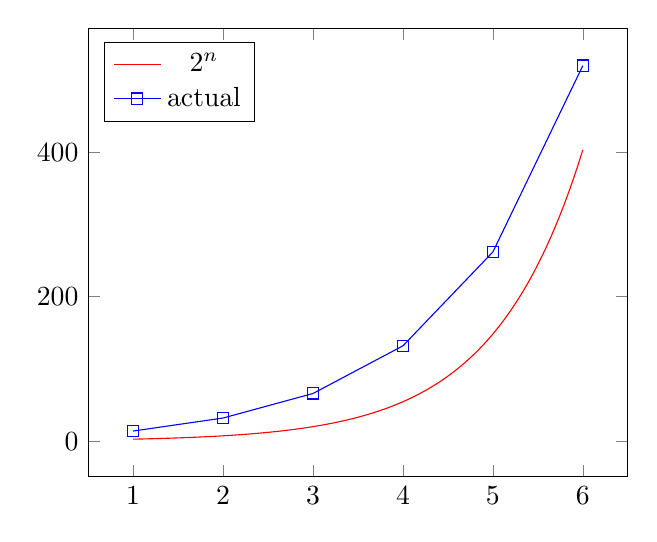
\begin{tikzpicture}
    \begin{axis}[
        legend pos= north west
        ]
       \addplot[
            domain=1:6,
            samples=100,
            color=red
        ]{exp(x)};
        \addlegendentry{$2^n$}

        \addplot[
            color=blue,
            mark=square
        ]
        coordinates {
(1,14)  (2,32)  (3,66) (4,132) (5,262) (6,520)
        };
        \addlegendentry{actual}

        %\addplot[
            %color=green,
            %mark=triangle
        %]
        %coordinates {
%(1,47)  (2,78) (3,128) (4,211) (5,347) (6,570)
        %};
        %\addlegendentry{fitted}

   \end{axis} 
\end{tikzpicture}
    \caption{Plot of type variables in Hindley-Milner type systems}
    \label{fig:expplot}
\end{figure}

\section{Higher level type systems}
The Hindley-Milner type system can only express relatively simple programs which robs algorithmic elegance in respect to other type systems.
One domain of programs that Hindley-Milner cannot express are those that rely on \textit{rank-n types}.
Rank-n types deals with letting abstractions have polymorphic parameters such that a type can be quantified within another type, having its depth bounded by n (rank-\textbf{n}).
For instance \autoref{lst:rankn} is not typable in Hindley-Milner since its type is \texttt{$\forall\tau$.($\forall\gamma$.$\gamma \rightarrow$ Int) $\rightarrow \tau \rightarrow$ Int}.
\begin{lstlisting}[language=ML,caption={Program that requires rank-n types},label={lst:rankn},mathescape=true]
fun f makeNum a =
    ((makeNum a) + (makeNum 0)) + (makeNum (0 == 2))
\end{lstlisting}
More generally, any type which is quantified on the left side of $\rightarrow$ cannot be moved out thus increases the rank.

Even languages which are typed and inferred by Hindley-Milner like Ocaml have introduced kinds through modules to allow higher-kinded types.
Hindley-Milner is in fact a restricted version of another more general type system called \textit{System F} (and System F\underline{$\omega$}).
The Hindley-Milner type system introduces abstractions as monomorphic types whereas System F allows any type to be polymorphic.
It turns out that allowing higher rank polymorphism makes type inference (type reconstruction in older literature) \textit{undecidable}~\cite{wells1999typability}.
\begin{remark}
    Formal type systems are in their essence deductive systems, which have provable properties such as \textit{decidability}.
    Decidability in deductive systems is a property which expresses whether a system can be decided by an algorithm (which relates to the encoding of algorithms on theoretic computers).
    If and only if every valid formula (type) in the deductive system (type system) can have its correctness decided (and reconstructed if necessary) algorithmically.
\end{remark}

Another variant of type system is \textit{System F\underline{$\omega$}}.
System F\underline{$\omega$} introduces another feature (System F\underline{$\omega$} is different to System F, it is not an extension) called type constructors.
It is uncommon to use System F\underline{$\omega$} on its own since it only allows type constructors of monomorphic types (System F introduces polymorphism), which does not yield much expressiveness since only specific types such as \texttt{Int $\rightarrow$ List Int} would be expressible.
Throughout this chapter, type constructors have already been introduced in such a way that they can occur in Hindley-Milner though algebraic data types such as \texttt{$\forall$a.a $\rightarrow$ List a}.
Very commonly, moderately generalized types need both the higher rank polymorphism implied by System F and the type constructors implied by System F\underline{$\omega$}.

Hindley-Milner can only take advantage of System F\underline{$\omega$} for rank 1 types which significantly constrains the generalization level.
A more expressive version of Hindley-Milner is System F$\omega$ which in fact, is the basis for the type system of Haskell, which is significantly more expressive than Hindley-Milner.
\begin{remark}
    Haskell has introduced some additional tweaks to System F$\omega$ to avoid the decidability problem among others.
\end{remark}

In more expressive functional programming language type systems it has become increasingly popular abstract over implementations by introducing concepts from \textit{category theory}.
Naturally many abstractions of category theory require rank-2 polymorphism.
More generally the larger the level of polymorphism allowed the larger the possible abstraction level becomes.
For instance a general purpose \textit{functor} is implementable and usable with rank-2 polymorphism while a natural transformation becomes a matter of rank-3 polymorphism.
\begin{remark}
    A functor is a mapping that maps from type constructor instance to another, which for instance can be a functor for lists which provides the algebra \texttt{$\forall$a.$\forall$b.List a $\rightarrow$ List b}.
\end{remark}
\noindent To generalize functor one must be able to express \textit{kinds} which are the types of type constructors denoted $* \rightarrow *$ for a type constructor that takes some type $*$ and creates some type $*$.
$* \rightarrow *$ is a unary type constructor whereas $*$ is an atomic type like \texttt{Int} or \texttt{List Int}, since these types are fully applied.
Kinds allow partial application on type constructors on a general level, since the only specific constraint is the shape and not where variables appear.
The relaxation of type constructions allow various types to be generalized such as \texttt{a $\rightarrow$ b $\rightarrow$ M a b} which could also have the signature of \texttt{a $\rightarrow$ b $\rightarrow$ M b a} which kinds abstract over generalizing $M$ to $* \rightarrow * \rightarrow *$.
The kind for \texttt{List} is $* \rightarrow *$ such that for any $\tau$ with kind $* \rightarrow *$ the type for functor map is \texttt{$\forall\tau$.($\forall$a.$\tau$a) $\rightarrow$ ($\forall$b.$\tau$b)}.
\begin{remark}
    Kinds are an abstraction which can exist purely theoretical without robbing the type system of expressiveness.
    Just as some complications in type systems are resolved with weakening the type system or enriching the syntax, kinds can bu abstracted away into types~\cite{weirich2013system}.
\end{remark}

$\lambda$P introduces \textit{Dependent types} which lets types depend on terms in the language.
A common example to show what dependent types can do is that of combining two lists $v_1$ and $v_2$ of size $n_1$ and $n_2$ into a list $v_3$ of size $n_1 + n_2$, where the size can be expressed in the type system.
The signature for such a function in $L$ could be \texttt{$\forall a.$List $n_1$ a $\rightarrow$ List $n_2$ a $\rightarrow$ List $(n_1 + n_2)$ a}.
Clearly one would have rules for lists such as a base case for the empty list \texttt{fun empty = Nil} with type \texttt{$\forall a.$List 0 a}, which indicates how the type system is lifted to a logical proofing tool.

\begin{figure}
    \centering
    \begin{tikzpicture}
        \matrix (m) [matrix of math nodes,
        row sep=3em, column sep=3em,
        text height=1.5ex,
        text depth=0.25ex]{
                    & \lambda\omega             &              & \lambda\Pi\omega             \\
        \lambda 2   &                           & \lambda\Pi 2                                \\
                    & \lambda\underline{\omega} &              & \lambda\Pi\underline{\omega} \\
        \lambda{\to}&                           & \lambda\Pi  \\
        };
        \path[-{Latex[length=2.5mm, width=1.5mm]}]
        (m-1-2) edge (m-1-4)
        (m-2-1) edge (m-2-3)
                edge (m-1-2)
        (m-3-2) edge (m-1-2)
                edge (m-3-4)
        (m-4-1) edge (m-2-1)
                edge (m-3-2)
                edge (m-4-3)
        (m-3-4) edge (m-1-4)
        (m-2-3) edge (m-1-4)
        (m-4-3) edge (m-3-4)
                edge (m-2-3);
    \end{tikzpicture}
    \captionsetup{singlelinecheck=off}
    \caption[nothing, items]{
        \begin{itemize}
            \item$\lambda\rightarrow$ is the simply typed lambda calculus without polymorphism.
            \item$\lambda\underline{\omega}$ is System F\underline{$\omega$}.
            \item$\lambda 2$ is System F.
            \item$\lambda\omega$ is System F$\omega$.
            \item$\Pi$ introduces \textit{dependent types} which is beyond the scope of this thesis.
        \end{itemize}
    }
    \label{lambdacube}
\end{figure}
\autoref{lambdacube} shows the \textit{lambda cube}, introduced in \cite{barendregt1991introduction} which encapsulates the family of formal type systems.
Complicated type system such as the \textit{calculus of constructions} ($\lambda\Pi\underline{\omega}$) are used in proof assistants since they essentially are deduction systems.
\section{Concluding remarks}
This section should act as an introduction to more general type systems and where Hindley-Milner is placed on the type system map.
Hindley-Milner is a small part of a larger more general system which has significant impact on the extensibility of Hindley-Milner.
Some very renown functional programming languages began by implementing Hindley-Milner as their type system since it is very fast in practice and relatively simple to implement.



\end{document}
